\chapter{A computational model for accentedness perception with L1 information}
\label{both_l1_l2}

\section{Introduction}

This chapter will use the knowledge derived from previous chapters, and propose a new scheme for automatic accentedness evaluation system. The system features a novel acoustic feature extraction process, which not only combines both segmental and suprasegmental information but also integrates speakers' L1 information. The way of adding L1 information in this study is also novel in automatic accentedness evaluation literature except for one study. \cite{moustroufas2007automatic} used utterance-level pronunciation scores extracted from both L1 and L2 acoustic models, calculated frame-wise and averaged over the utterance. However, the proposed system has an important difference: the pronunciation scores are calculated on phoneme segments and provide more specific information regarding the accentedness of different phonemic categories. Suprasegmental acoustic measurements representing speech prosody are also included. Furthermore, \cite{moustroufas2007automatic} assume the human evaluator can speak both L1 and L2 and experiments were conducted on only one L1. This study wants to investigate if the L1 acoustic model can help improve prediction even if the human evaluators have no knowledge of the underlying L1.

To validate the proposed system, the dataset introduced in chapter \ref{sec:methodology} will be employed again to conduct experiments on automatic accentedness evaluation both L1-dependently and L1-independently. Same leave-one-speaker-out CV will be used to evaluate the performance of the system. Finally, possible extensions and improvements over the state-of-the-art systems are discussed.

\section{Method}

\begin{figure}[t]
        \begin{minipage}[t]{1.0\linewidth}
        \centering
            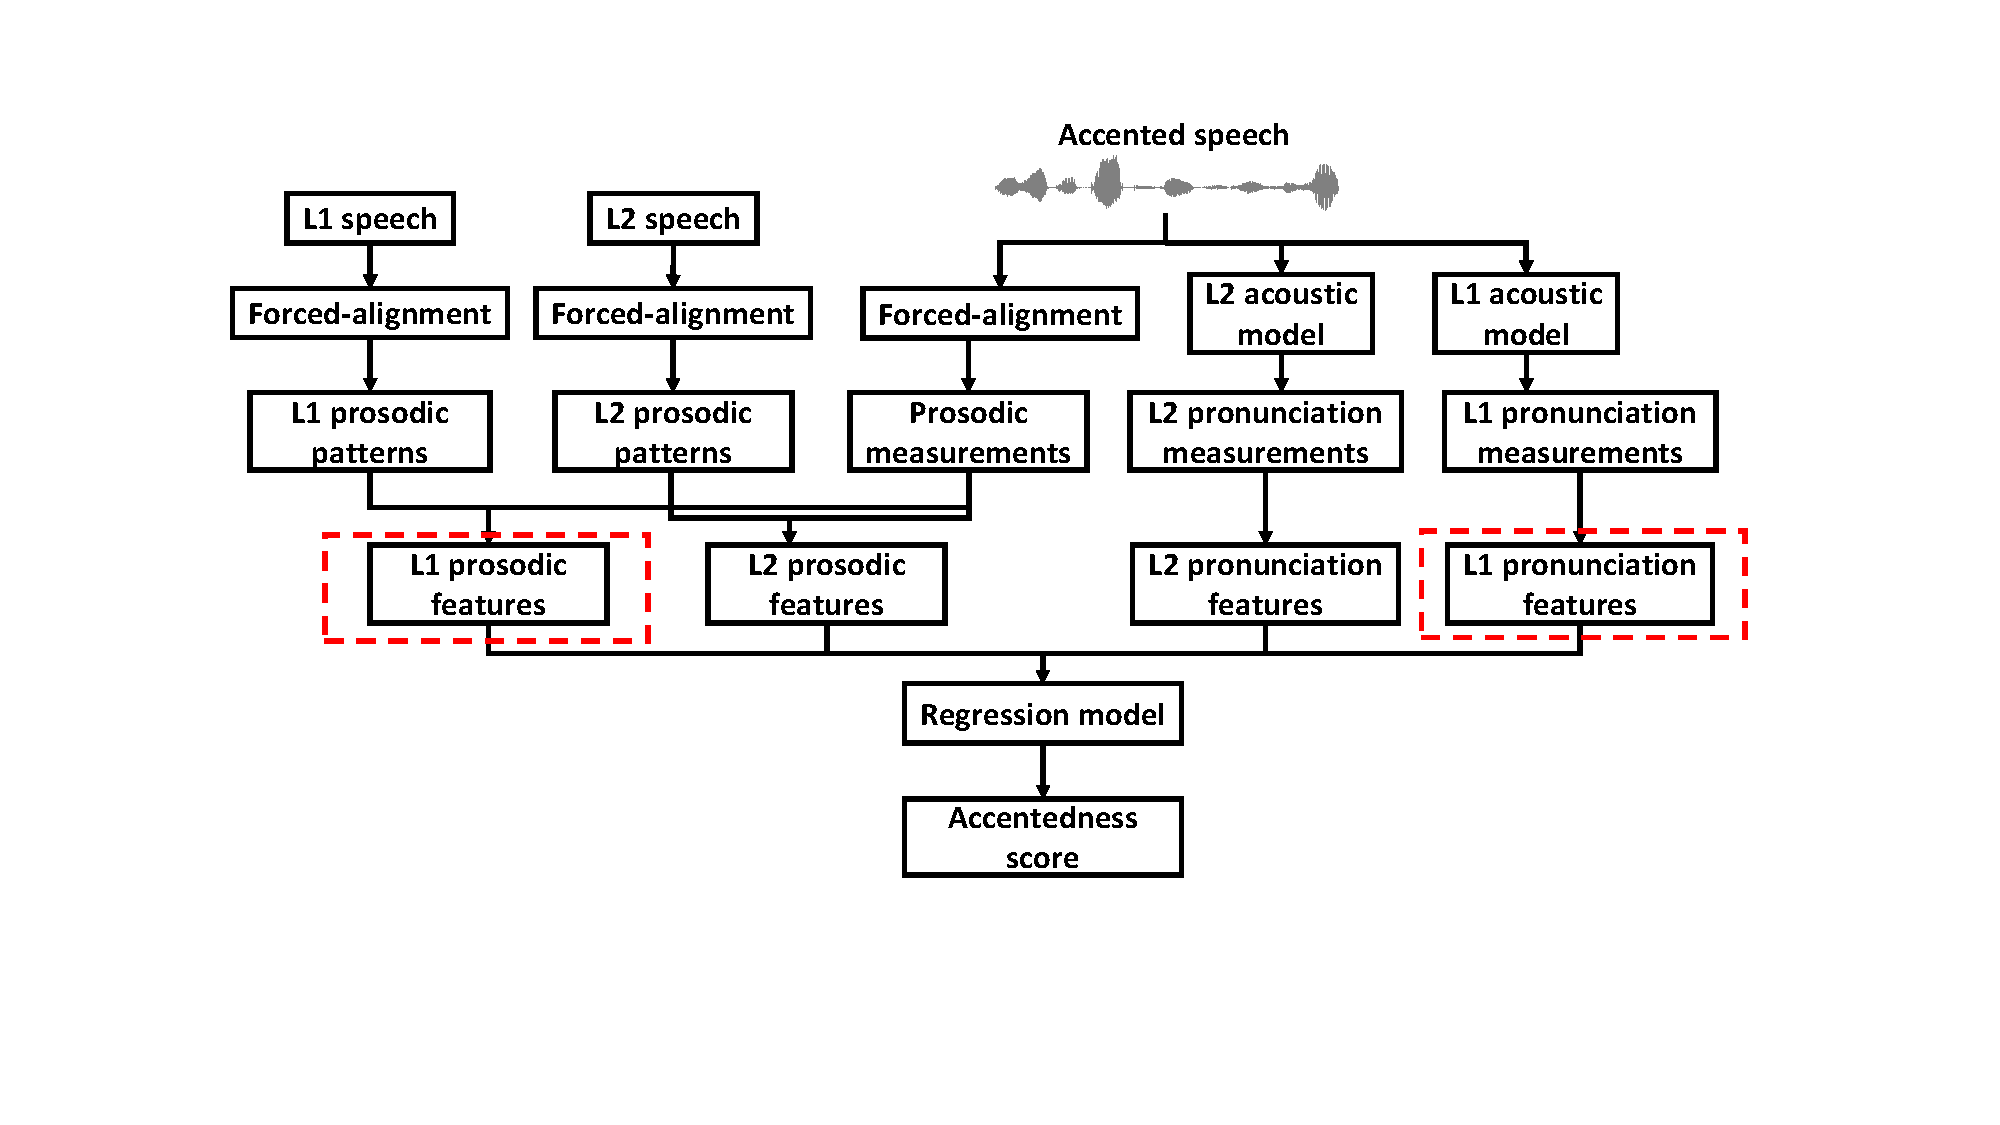
\includegraphics[width=5.0in]{figures/AAE_diagram.pdf}
        \end{minipage}%
        \caption{Diagram of the proposed computational model. The blocks within red box are the highlights of the current model.}
        \centering
        \label{fig:aae_diagram}
     \end{figure}

The diagram of the proposed computational model is shown in figure \ref{fig:aae_diagram}. Prerequisites include a well trained acoustic model (hybrid system built on GMM-HMM or DNN-HMM) on native L2 speech, a well trained acoustic model on native L1 speech, a corpus of native L2 speech for extracting L2 prosodic patterns and a corpus of native L1 speech for extracting L1 prosodic patterns. First, accented speech in L2, native L1 speech and native L2 speech are processed with forced-alignment tools to obtain the durations of each phoneme in the transcripts. There are many available forced-alignment tools with open access \footnote{As summarized in \url{https://github.com/pettarin/forced-alignment-tools}}. Some of them support forced-alignment for multiple languages. For accented speech, usually the forced-alignment performance is inferior compared to native speech because those tools also use acoustic models trained on native speech. To relieve this problem, some recent studies trained the acoustic models for accented speech forced-alignment directly on accented speech to achieve data matching \citep{tao2016exploring, qian2017bidirectional}. However, it requires huge amount of non-native speech recordings which is usually inaccessible. This study employs a forced-alignment tool with an acoustic model trained on a native English speech corpus with about 1000 hours training data to get the phonemes durations of accented speech. After obtaining the phoneme durations of native L1 speech, native L2 speech and accented speech, the feature extraction procedure introduced in section \ref{sec:supraseg} will be applied to get the prosodic patterns of native L1 and L2. This can be achieved by averaging over the sentence-level features over all native L1 and L2 utterances. At the same time, prosodic feature vectors of each accented speech utterances are saved for following process. What previous studies have investigated is that computing the difference between prosodic measurements of accented speech and native L2 speech gives the deviation from native prosodic patterns. This study improves this by adding the difference between prosodic measurements of accented speech and native L1 speech to represent how much the prosodic patterns of accented speaker are affected by L1. This results in two sets of suprasegmental feature vectors for each accented speech utterance.

In parallel, accented speech recordings are also sent to both L1 and L2 acoustic models to get the pronunciation scores of each phoneme in the utterance based on the corresponding acoustic model. The algorithms proposed in section \ref{sec:segmental} are used to convert phoneme-level pronunciation score to sentence level pronunciation measurements. Different from previous studies in the literature, this study not only measures the pronunciation mismatch with native L2 speech but also how much the pronunciation in L2 is affected by the speaker's L1. This again results in two sets of segmental feature vectors for each accented speech utterance. Up to now, there are four feature sets for each accented speech utterance. All of them can be concatenated to form a larger feature vector. Feature vectors without L1 information will be used as baseline system in this study, which has been adopted by recent studies \citep{black2015automated, tao2016exploring, qian2017bidirectional}.

Almost all studies in literature treat the accentedness (or nativeness) evaluation as a regression problem. With the developed sentence-level features, each speaker becomes a data sample with a labeled accentedness score. The accentedness score can be on different scales depending on tasks. This study use a 4-point scale to annotate the accentedness score. Usually, the label will be the average of multiple annotators to reduce inter-rater variability. With feature representation and labels, a regression model can be trained to learn the mapping from input feature to accentedness score. Considering the relatively small number of speakers, this study adopts ridge regression (linear regression with L2-norm regularization) together with a simple feature selection algorithm based on univariate regression analysis. Depending on the dataset, different regression models can be used to achieve better performance. For example, support vector regression \citep{black2015automated}, Gaussian process \citep{grosz2015assessing}, random forest \citep{qian2017bidirectional} and Deep neural networks \citep{grosz2015assessing} are also used in previous studies. SVR is also tried in this study but it is not better than linear regression.

To evaluate the proposed systems, experiments are conducted on both L1-dependent and L1-independent tasks. For L1-dependent task, the system is built on speakers from one L1; for L1-independent task, the system is built on speakers from different L1s. In both cases, leave-one-speaker-out CV is used to evaluate the system's performance because leave-one-out CV is almost the unbiased estimate of generalization error \citep{elisseeff2003leave}. As previous chapters, PCC and MAE on all speakers are used as performance indicators.

\section{Results}

\begin{table}[t]
\centering
\caption{Performance of accentedness score prediction with different feature sets for different L1s. ``L2\_seg'' stands for L2 pronunciation features. ``+L1\_seg'' means adding L1 pronunciation features to original L2 pronunciation features. ``L2\_supraseg'' stands for L2 prosodic features; ``+L1\_supraseg'' means adding L1 prosodic features to original L2 prosodic features. ``L2\_seg+L2\_supraseg'' represents combining both L2 pronunciation features and L2 prosodic features. ``L1,2\_seg+L1,2\_supraseg'' represents combining all four sets of features together.}
\label{table:ch6_l1_ind}
\resizebox{\columnwidth}{!}{%
\begin{tabular}{|l|c|c|c|c|c|c|c|c|}
\hline
\multicolumn{1}{|c|}{\multirow{2}{*}{}} & \multicolumn{4}{c|}{PCC} & \multicolumn{4}{c|}{MAE} \\ \cline{2-9}
\multicolumn{1}{|c|}{} & German & French & Mandarin & Spanish & German & French & Mandarin & Spanish \\ \hline
L2\_seg & 0.734 & 0.254 & 0.707 & 0.681 & 0.204 & 0.406 & 0.343 & 0.535 \\ \hline
\hspace{0.5cm}+L1\_seg & 0.833 & 0.411 & 0.727 & 0.730 & 0.163 & 0.370 & 0.329 & 0.464 \\ \hline
L2\_supraseg & 0.583 & 0.647 & 0.581 & 0.698 & 0.202 & 0.310 & 0.425 & 0.507 \\ \hline
\hspace{0.5cm}+L1\_supraseg & 0.772 & 0.680 & 0.712 & 0.729 & 0.180 & 0.289 & 0.380 & 0.482 \\ \hline
L2\_seg + L2\_supraseg & 0.494 & 0.667 & 0.733 & 0.846 & 0.251 & 0.308 & 0.319 & 0.404 \\ \hline
L1,2\_seg+L1,2\_supraseg & 0.590 & 0.709 & 0.771 & 0.898 & 0.225 & 0.277 & 0.296 & 0.341 \\ \hline
\end{tabular}}
\end{table}

Table \ref{table:ch6_l1_ind} shows the performance of accentedness score prediction in L1-dependent way with different feature sets. Part of the results is from table \ref{table:seg_pred} and \ref{table:supraseg_pred}. The results on German speakers are achieved with the 18-speaker subset, and all 30 French speakers are used here. The results show that when combining both segmental and suprasegmental features, the performance is better than either only using segmental features or only using suprasegmental features. For Spanish speakers, the improvement is the largest. However, this observation does not hold for German speakers: the performance degrades a lot after combining both segmental and suprasegmental features. Possible reasons for this could be model overfitting considering there are only 18 data samples, resulting in worse prediction accuracy when combining two feature sets. This problem can be relieved by using an ensemble of two ridge regression model trained on segmental and suprasegmental features separately. Actually, when applying a weighted sum on the predictions of segmental model and suprasegmental model, the correlation and MAE are 0.791 and 0.171 respectively, which are better than single model. To keep the results consistent, only performance on feature-level fusion are presented. When adding L1 related information to the feature sets, the prediction accuracy is further improved for all four L1s. For Spanish speakers, the PCC is as high as 0.9 (but the MAE is also the highest). Again, the ensemble model performance of German speakers is 0.890 for PCC and 0.137 for MAE, which are also big improvement compared to model trained without L1-related features. This improvement is expected based on the results shown in previous two chapters.

\begin{figure}[t]
        \begin{minipage}[t]{1.0\linewidth}
        \centering
            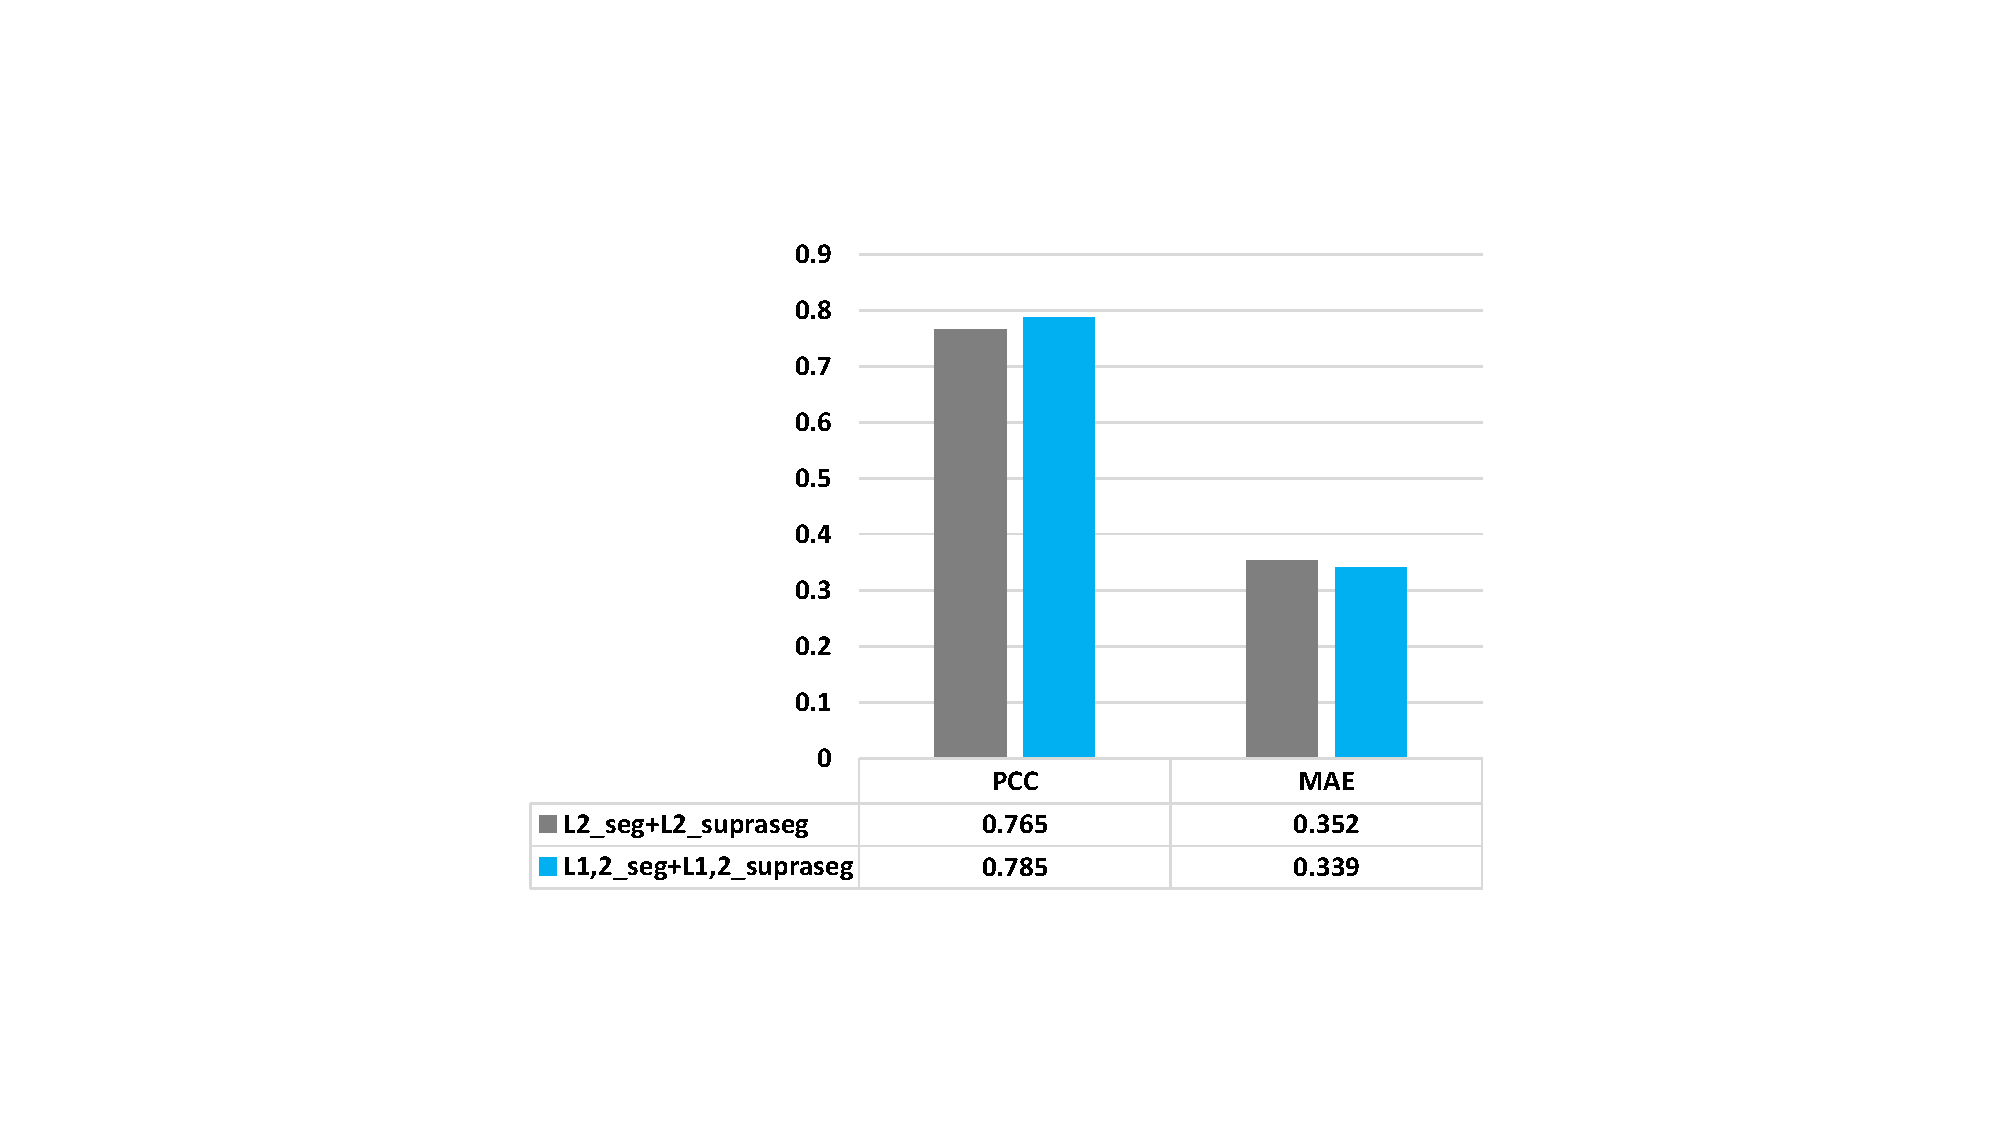
\includegraphics[width=5.0in]{figures/allspk_results.pdf}
        \end{minipage}%
        \caption{Bar plots and detailed values of results in L1-independent way.}
        \centering
        \label{fig:allspk_results}
     \end{figure}

%     \begin{figure}[t]
%        \begin{minipage}[t]{1.0\linewidth}
%        \centering
%            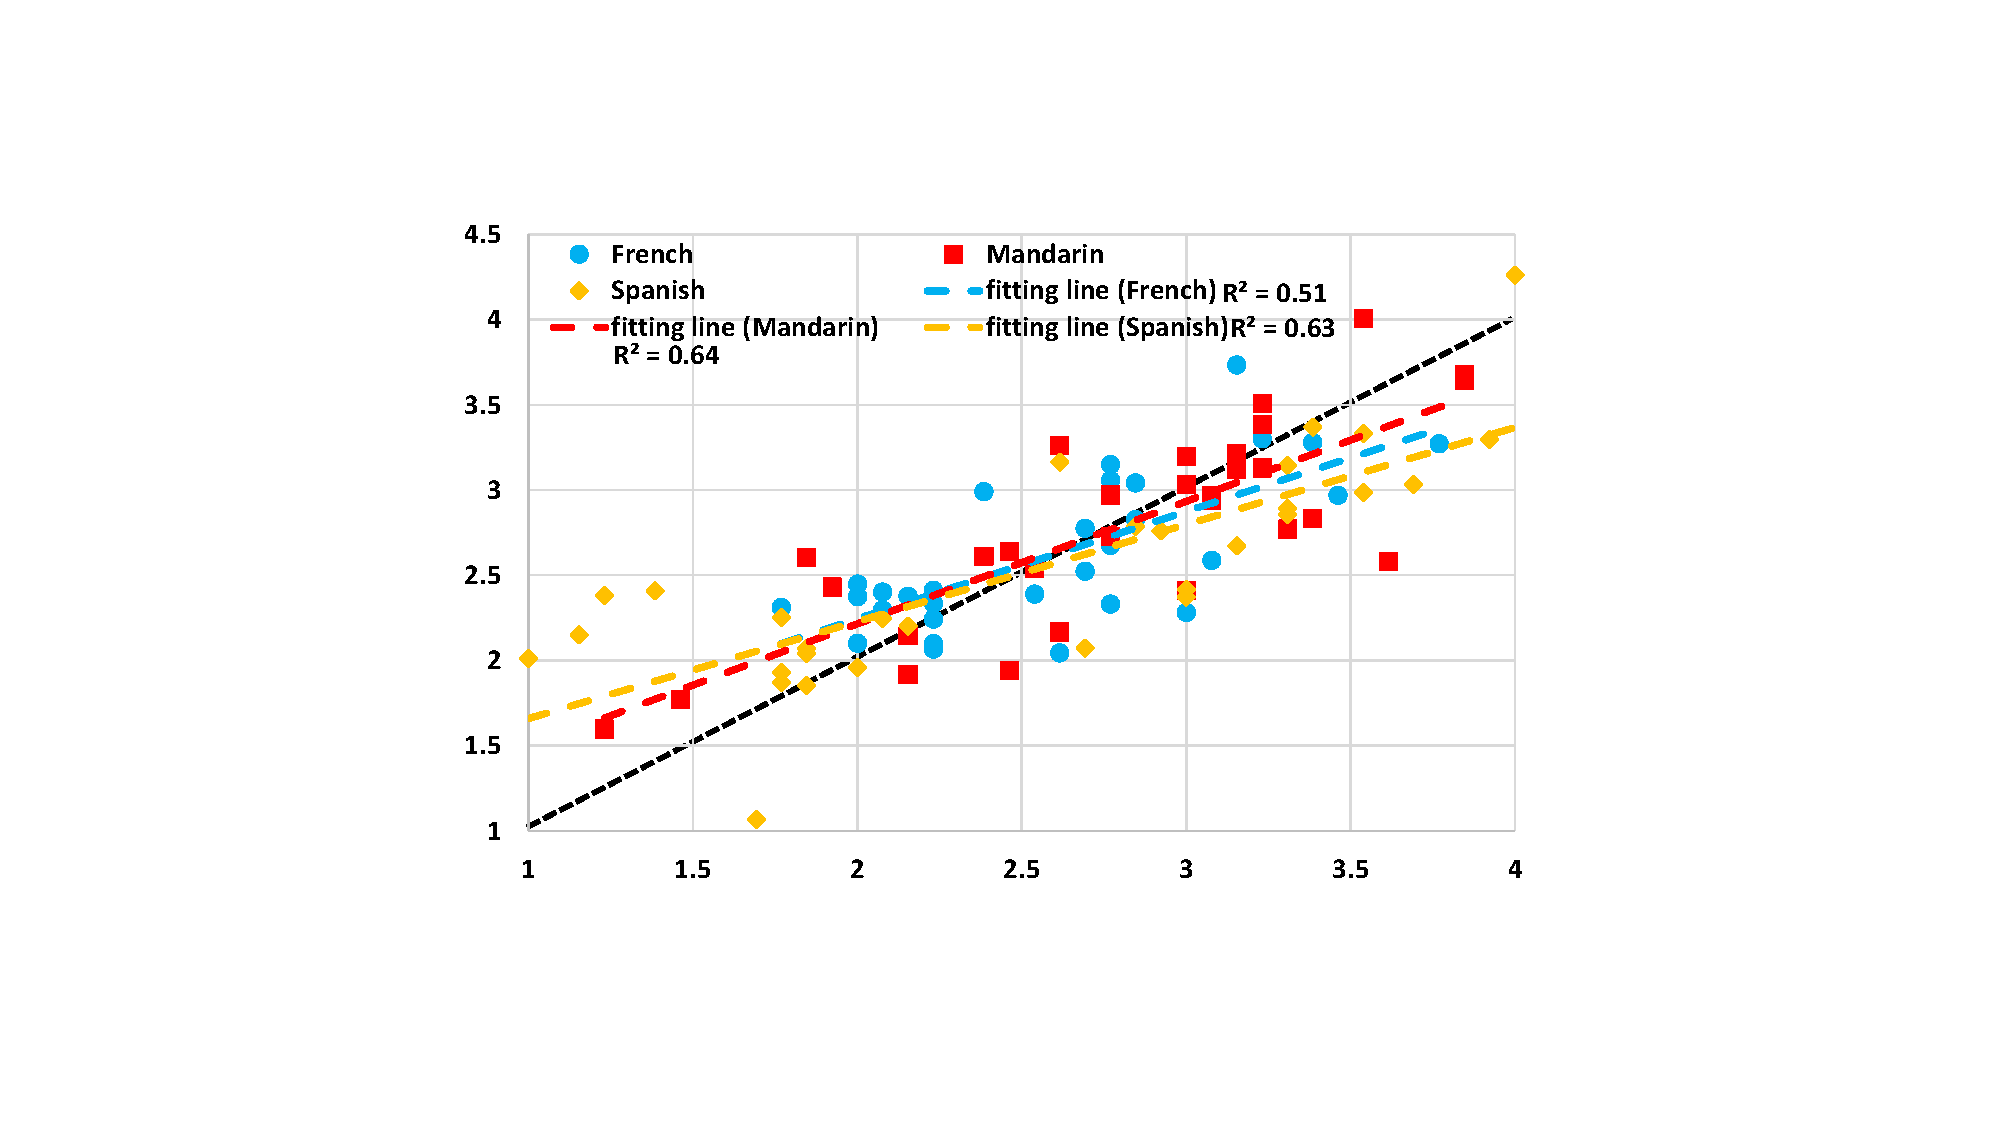
\includegraphics[width=5.0in]{figures/allspk_results_scatter.pdf}
%        \end{minipage}%
%        \caption{Scatter plots of the true labels and predictions of all 90 speakers from different L1s (French speakers in blue circles, Mandarin speakers in red squares and Spanish speakers in yellow diamonds). X axis is the groundtruth accentedness score and Y axis is the prediction. The fitting line for each L1 is also shown here together with the perfect fitting line (black dash line). R square values are also presented.}
%        \centering
%        \label{fig:allspk_results_scatter}
%     \end{figure}

\begin{figure}[t]
        \begin{minipage}[t]{1.0\linewidth}
        \centering
            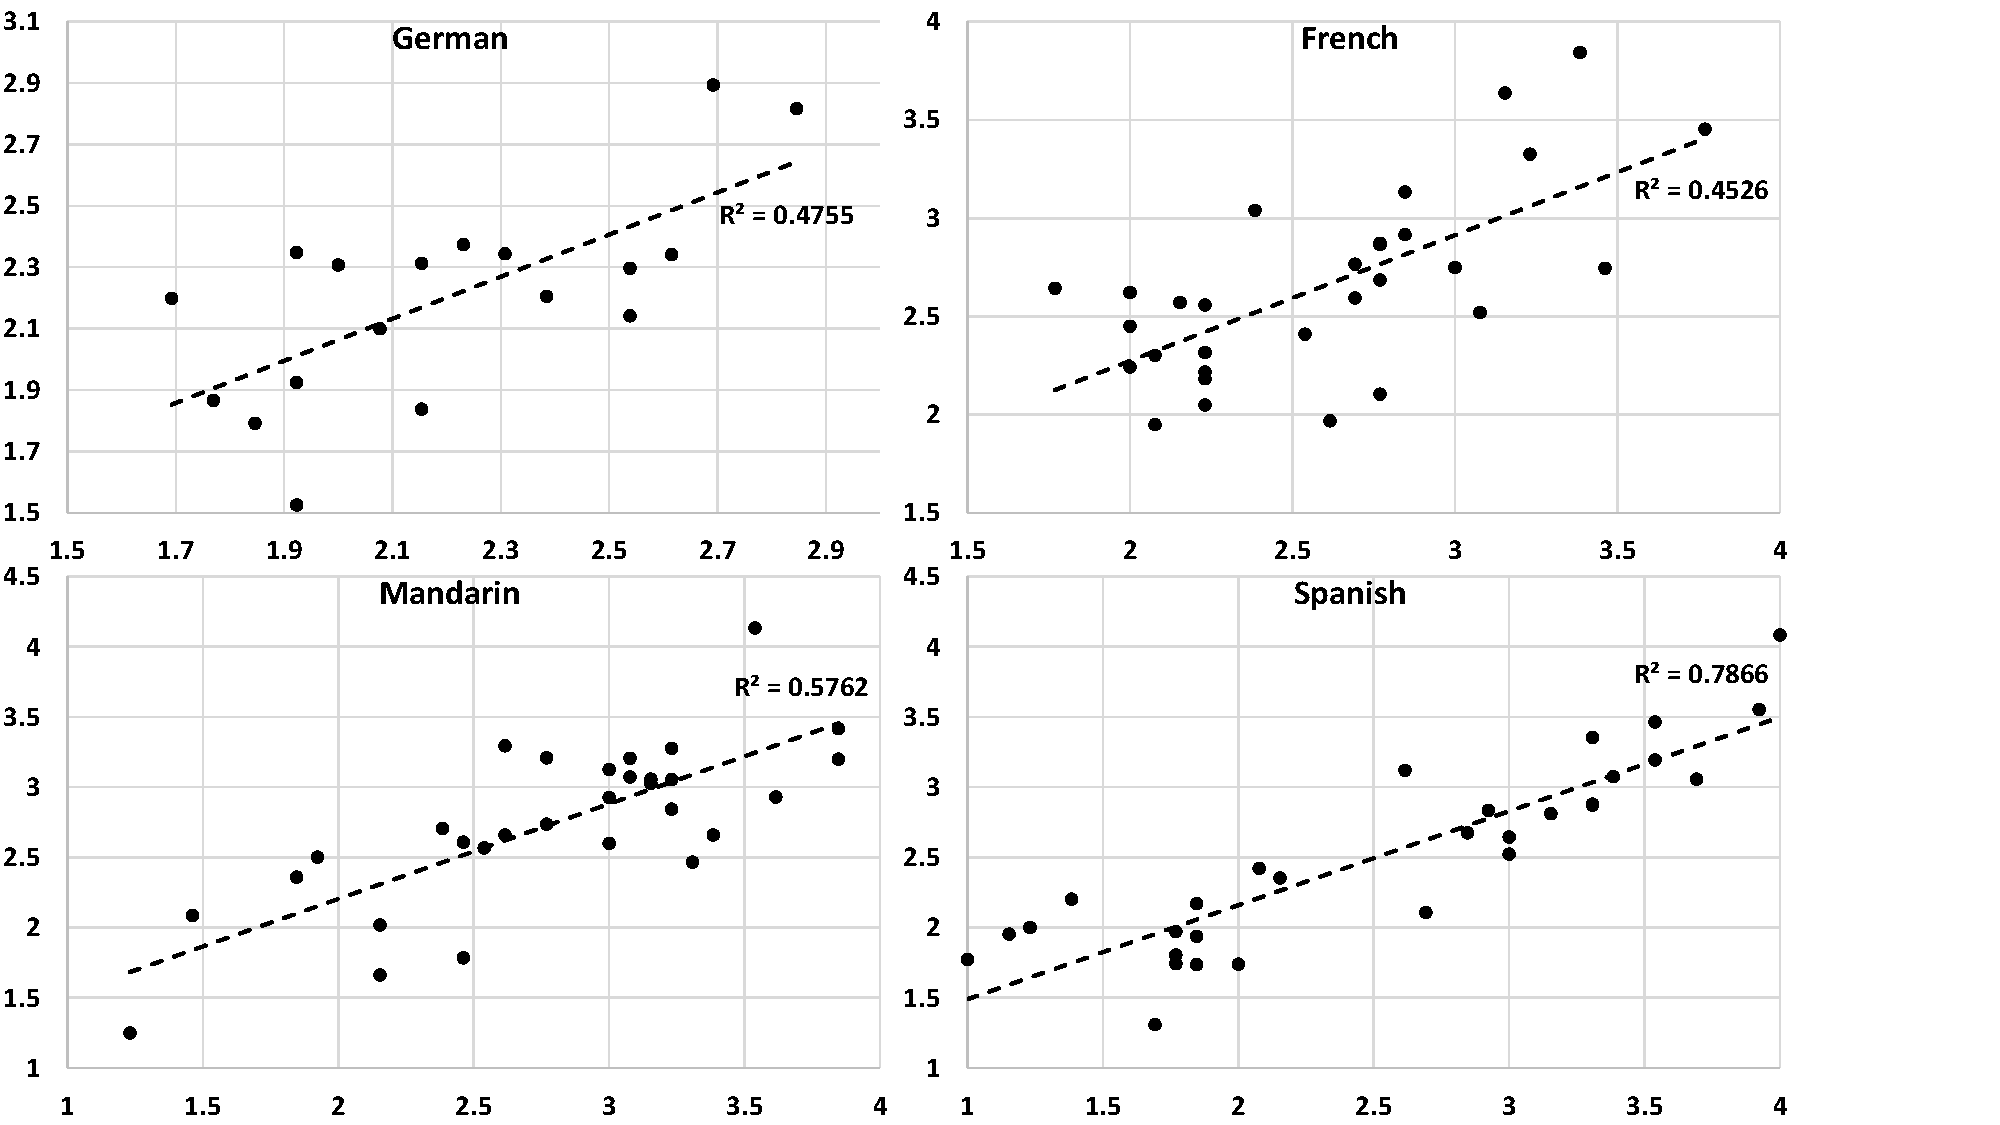
\includegraphics[width=5.0in]{figures/allspk_results_scatter_L1s.pdf}
        \end{minipage}%
        \caption{Scatter plots of the true labels (X-axis) and predictions (Y-axis) of speakers from different L1s. The fitting line for each L1 is also shown here together with the R-squared values.}
        \centering
        \label{fig:allspk_results_scatter}
     \end{figure}

Figure \ref{fig:allspk_results} shows the results when all speakers from German (18-speaker subset), French, Mandarin and Spanish are taken into account. Improvement over baseline model (employed in current state-of-the-art automatic accentedness evaluation system) without L1-related features can be observed when adding L1-related features to the input, although the improvement is relatively marginal compared to L1-dependent experiments. It proves that the L1 related information can also help the prediction in L1-independent case. However, it can be found that the improvement in L1-independent experiment is less than the improvement in L1-dependent experiment. The reason for this will be discussed in next section. Since the improvement is not that large, figure \ref{fig:allspk_results_scatter} only shows the scatter plots achieved with all four feature sets for different L1s. Speakers from different L1s are plot individually with fitting lines and R-squared values. It can be found that Spanish speakers are fitted the best with the highest R-squared value. German and French speakers are not fitted well compared to Spanish and Mandarin speakers. The overall correlation coefficient is 0.811 as shown in figure \ref{fig:allspk_results}, which indicates a strong relationship between model predictions and groundtruth accentedness scores.

\section{Discussion}

This chapter derives a computational model for automatic accentedness evaluation based on findings in previous chapters. The core idea is a new feature extraction scheme that not only quantifies the deviation from native L2 phonological patterns but also how much the accented speech is affected by L1 phonological patterns. Experiments on both L1-dependent and L1-independent tasks show that there is consistent improvement when combining L1 information in the input feature sets.

As a computational model, some blocks of the proposed system can be flexible depending the specific task and resources available. For example, more powerful acoustic models can be used to derive better pronunciation features. More accurate forced-alignment can also be achieved with better forced-alignment tools, thus improving the prosodic features. Depending on the size of dataset, regression models with different complexity can be applied to achieve better performance. Although the evaluation in the current study is done on speaker-level, the proposed framework can be easily extended to sentence-level evaluation.

As mentioned before, the performance improvement of the proposed system on L1-independent tasks is smaller than L1-dependent tasks. This is due to the variability introduced by different L1 acoustic models and different forced-alignment tools for different L1s. This may result in the scales of L1 related features variate for different L1s. This problem can be relieved by using equally powerful L1 acoustic models and forced-alignments, although it could cost much more effort. Another possible solution is to normalize the L1-dependent features with the distance between L1 and L2 pronunciation patterns or the distance between L1 and L2 prosodic patterns. It is not easy to directly calculate the distance between pronunciation patterns of two language given their acoustic models. This study tried to normalize the L1 prosodic measurements with the distance between prosodic patterns of L1 and L2, which almost does not change the final results. This is possibly because there is too much variation of the forced-alignment quality of different L1s. However, this study still believe this is a direction worth more investigation.
